\chapter{Background}\label{section:background}
\thispagestyle{myheadings}

	In this section, I will go over the building blocks required to construct the outsourced database systems and their components that I will discuss in the next chapters.
	These prerequisites include the symmetric encryption, \acrshortpl{oram} and PathORAM \cite{path-oram} in particular, \acrlong{dp} and \acrshort{dp} sanitizers, and finally, \acrlongpl{tee}.
	\emph{Some of the following sections were paraphrased or taken verbatim from my published work \cite{ore-benchmark-17,epsolute}.}

	\section{Symmetric encryption}\label{section:background:encryption}

		Symmetric encryption scheme is a tuple of algorithms $\algo{E} = \{ \algo{KeyGen}, \algo{Enc}, \algo{Dec} \}$ with the following properties.
		$\algo{E.KeyGen} \left( \secparam \right) \to \key$ is a \emph{randomized} algorithm that on a security parameter $\secparam$ returns a key that will be used for both encryption and decryption.
		$\algo{E.Enc} \left( m \right) \to c$ is a \emph{randomized} algorithm that on a plaintext message $m \in \bin^*$ produces its ciphertext $c \in \bin^*$.
		$\algo{E.Dec} \left( c \right) \to m$ is a \emph{deterministic} algorithm that on a ciphertext $c \in \bin^*$ produces its original plaintext message $m \in \bin^*$.

		\subsection{Security}

			The security of the symmetric encryption is typically defined as the indistinguishability under a certain attack.
			The definition is structured around the game between the challenger and the adversary \adversary{}.
			The challenger fixes one of the two ``worlds'', left or right, and the adversary wins the game if she can reliably tell which world it was.

			A weaker security definition, \acrfull{ind-cpa}, intuitively, requires that the ciphertext leaks nothing about the plaintext.
			To formalize the requirement, the adversary can give the challenger a set of plaintext pairs to encrypt, and the challenger responds with a set of ciphertexts where the left or the right part was encrypted.
			The adversary can then use any (polynomial) algorithm over the ciphertexts and make a guess of whether the left or the right part was encrypted.
			The claim is, if there is anything that the ciphertext leaks about the plaintext, there exists an adversary who will win.
			The security claim is therefore contrapositive --- the scheme is \acrshort{ind-cpa} secure iff there is no such adversary that wins the game.
			The \acrshort{ind-cpa} definition can be upgraded to allow the adversary to choose the plaintexts adaptively (\acrshort{cpa}2), or require the ciphertext be indistinguishable from a random bit-string (\acrshort{cpa}\$).

			\acrshort{ind-cpa} security is not by itslef sufficient since it does not account for the decryption part of the scheme.
			There are known attacks that decrypt the plaintext (i.e., defeat the encryption) if the adversary can trigger the decryption and observe the process or the result (see padding attack \cite{padding-attack} and \acrshort{xml} encryption attack \cite{xml-break-encryption}).

			The stronger definition, \acrfull{ind-cca}, captures the decryption component.
			It extends the \acrshort{ind-cpa} game in that the adversary can now request the challenger to decrypt \emph{any} ciphertext of her choice \emph{except} the ones that the chalenger himself encypted for the adversary.
			The adversary still outputs a guess of the two worlds and wins if reliably guesses correctly.
			Note that in this game if the decryption can fail for any reason, or even if \adversary{} can observe any difference in execution for different inputs, the scheme is insecure.
			Therefore, \acrshort{ind-cca} immediately rules out the aformentioned attacks \cite{padding-attack,xml-break-encryption}.
			Similarly to \acrshort{ind-cpa}, \acrshort{ind-cca} also has the adaptive and indistinguishable\hyp{}from\hyp{}pseudorandom variants \acrshort{cca}2 and \acrshort{cca}\$.

		\subsection{Components}

			Note that for the practical purposes I define the encryption algorithm as randomized --- producing different ciphertext for the same plaintext on every invocation.
			While this is how the symmetric encryption scheme is used in applications, formally, producing the deterministic ciphertext and randomizing it are different operations.

			Internally, the encryption scheme typically consists of a keyed \acrfull{prp} (also known as a \emph{block cipher}), a \acrfull{prg} that is used to generate a (pseudo)random \acrfull{iv} and a block cipher \emph{mode of operation}.\footnote{% chktex 36
				Here I describe the \emph{block ciphers} family of symmetric encryption algorithms.
				Streaming ciphers are not used in this thesis.
			}
			First, the input $m \in \bin^*$ is split into blocks (depending on the underlying block cipher, for example, 128 bits) and the last block is padded if necessary.
			Second, the pseudorandom \acrlong{iv} of size of the block is generated with a \acrshort{prg}.
			Intuitively, this is the part that contributes the  ``randomness'' to the process.\footnote{
				There are some modes of operation that do not require the \acrlong{iv}, such as \acrfull{ecb} mode, but these are insecure.
			}
			Finally, the \acrshort{iv} is prepended to the plaintext blocks and the algorithm applies the permutation to one block at a time with the input masked according to the mode of operation.
			The resulting object is a ciphertext that is one block longer than a plaintext due to \acrshort{iv}.
			In practical systems, the ciphertext is then broken up into components, like the ciphertext material itself, the \acrshort{iv}, the version of the key, etc.
			Also note that the encryption scheme key has a maximum number of times it can be used for encryption (its \emph{operational lifetime}).

			\acrfull{aes} \cite{aes-nist} is a \acrshort{nist}-standardized block cipher, which, along with the standardized mode of operation \cite{nist-modes} and \acrshort{prg} \cite{nist-prg} used to generate the \acrshort{iv}, forms the symmetric encryption system.

	\section{\texorpdfstring{\acrlong{oram}}{Oblivious Random Access Machine}}\label{section:background:oram}

		Informally, \acrfull{oram} is a mechanism that lets the users hide their access pattern to remote storage.
		An adversarial server can monitor the actual accessed locations, but she cannot tell a read from a write, the content of the block or even whether the same logical location is being referenced.
		The notion was first defined by \textcite{oram-theory} and \textcite{oram-original}.

		More formally, a $(\eta_1, \eta_2)$-\acrshort{oram} protocol is a two-party protocol between a client \client{} and a server \server{} who stores a memory array.
		In each round, the client \client{} has input $(o, a, d)$, where $o$ is an access type (\oramRead{} or \oramWrite{}), $a$ is a memory address and $d$ is a new data value, or $\bot$ for read operation.
		The input of \server{} is the current array.
		Via the protocol, the server updates the memory or returns to \user{} the data stored at the requested memory location, respectively.
		We speak of a sequence of such operations as a program \oramProgram{} being \emph{executed under the \acrshort{oram}}.

		An \acrshort{oram} protocol must satisfy correctness and security.
		Correctness requires that \client{} obtains the correct output of the computation except with at most probability $\eta_1$.
		For security, we require that for every client \client{} there exists a simulator $\simulator_\oram$ which provides a simulation of the server's view in the above experiment given only the number of operations.
		That is, the output distribution of $\simulator_\oram (c)$ is indistinguishable from $\algo{View}_\server$ with probability at most $\eta_2$ after $c$ protocol rounds.
		Note that the \acrshort{oram} protocols typically differ in the way the storage is organized and manipulated, but are similar in that the records or blocks are symmetrically encrypted (see \cref{section:background:encryption}).

		\acrshort{oram} protocols are generally stateful, after each execution the client and server states are updated.
		\emph{For brevity, throughout the thesis I will assume the \acrshort{oram} state updates are implicit, including the encryption key generated and maintained by the client.}

		Some existing efficient \acrshort{oram} protocols are Square Root \acrshort{oram} \cite{oram-theory}, Hierarchical \acrshort{oram} \cite{oram-original}, Binary-Tree \acrshort{oram} \cite{binary-tree-oram}, Interleave Buffer Shuffle Square Root \acrshort{oram} \cite{shortest-path-oram}, TP-ORAM \cite{tp-oram}, PathORAM \cite{path-oram} and TaORAM \cite{taostore}.
		For detailed descriptions of each protocol, I recommend the work of \textcite{oram-survey-feifei}.
		The latter three \acrshortpl{oram} achieve the lowest communication and storage overheads, $\bigO{\log \dataSize}$ and \bigO{\dataSize}, respectively.

		\subsection{PathORAM}

			PathORAM \cite{path-oram} is one of the most commonly used \acrshort{oram} protocols due to its efficiency and simplicity.
			In this section I briefly describe this construction as it is used as an \acrshort{oram} instantiation in the rest of the thesis.

			In the PathORAM, both the client \client{} and the server \server{} are stateful.
			The server stores the encrypted records (blocks) grouped in buckets, and the buckets form a binary tree.
			The client's storage, although asymptotically linear in the data size, is relatively small in practice.
			The client stores the \emph{position map} that maps the record ID to a leaf in the server tree storage and a small amount of stash, which can store some plaintext blocks on the client side.

			The main invariant of the protocol is that at all times the ciphertext of the record $a$ is stored somewhere on the \emph{path} from the root to the leaf that is mapped to $a$, or in the stash (hence the name of the construction).

			The \acrshort{oram} is initialized with a binary tree of buckets with all buckets containing valid encryptions of dummy records.
			The position map is sampled at random (filled with permuted distinct numbers).

			Main routine of the \acrshort{oram} is an access sub-protocol, which is similar for read \oramRead{} and write \oramWrite{} type of access (remember, \acrshort{oram} hides the type of access from the curious server).
			In PathORAM, the access $(o, a, d)$ consists of four steps.
			First, remap the current leaf $x$ for $a$ to a new random leaf $x^\prime$.
			Second, read the entire path to leaf $x$ (all buckets from root to leaf) into the client stash.
			Third, the client updates the block value to $d$ if the access is a write \oramWrite{}.
			Finally, write back the path to leaf $x$ filling the buckets with all blocks from stash in a way that maintains the invariant.

			The newly updated block $a$ with the new value $d$ may be included in the new path, or it may stay in the stash.
			It is important that the stash size be provably bounded.
			\cite[Theorem 1]{path-oram} does exactly that --- at least for the bucket size of 5, the probability of stash overflow and its size are related as in \cref{equation:path-oram-stash}.
			\begin{equation}\label{equation:path-oram-stash}
				\probability{ \mathsf{stash\ size} > x } \leq 14 \cdot (0.6002) ^ x
			\end{equation}
			If the probability of a protocol failure is thought of as the adversary's advantage (the probability to break the security), then the stash size equivalent to 128-bit security is about 100 blocks for the bucket of size 5 \cite[Figure 5]{path-oram}.

	\section{\texorpdfstring{\acrlong{dp}}{Differential Privacy}}

		\acrfull{dp} is a guarantee on a mechanism that takes a dataset and returns some result.
		The guarantee states that for two neighboring databases (that differ in exactly one record), the probability that the adversary will understand by looking at the output, which of the two databases was used as an input, is bounded.
		More formally, the \acrlong{dp} is defined in \cref{definition:dp}.

		\begin{definition}[\acrlong{dp}, adapted from \cite{our-data-ourselves, differential-privacy-original}]\label{definition:dp}
			A randomized algorithm \algo{A} is $(\epsilon, \delta)$-differentially private if for all $\database_1 \sim \database_2 \in \searchKeyDomain^\dataSize$, and for all subsets $\mathcal{O}$ of the output space of \algo{A},
			\[
				\probability{ \algo{A}{ \database_1 } \in \mathcal{O} } \leq \exp(\epsilon) \cdot \probability{ \algo{A}{ \database_2 } \in \mathcal{O} } + \delta \; .
			\]
		\end{definition}

		One way to interpret this definition is the following.
		Probabilities are taken over the coins of algorithm \algo{A}, which answers a query based on a dataset.
		A natural instantiation of \algo{A} is a view of a distinguishing adversary \adversary{}, who tries to guess which of the two datasets was used.
		The expression in \cref{definition:dp} then bounds the advantage of \adversary{} with $\epsilon$ and $\delta$ parameters.
		Note that $\exp( x ) \approx 1 + x + \frac{x^2}{2!}$, and for sufficiently small $x$ the last term is negligible.
		If we put $\epsilon + 1$ in place of $\exp( \epsilon )$, it becomes clear that $\epsilon$ is the exact value by which two probabilities are allowed to differ.
		For $\epsilon = 0$, they have to be equal, for $\epsilon = 0.01$, probabilities may differ by \SI{1}{\percent}.
		Therefore, $\epsilon$ is called \emph{a privacy budget} of a \acrshort{dp} system.
		$\delta$ term is additive and therefore must be small by itself.
		This term is essentially a probability that the entire system fails.
		For example, if \algo{A} is a randomized algorithm that fails with a certain chance, this probability will be $\delta$.
		For instance, a PathORAM \cite{path-oram} algorithm can have a stash overflow with a bounded probability \cite[Theorem 1]{path-oram} and it will cause the entire algorithm to fail.
		If PathORAM is used in a \acrshort{dp} system then this probability, however small, bounded and negligible, will have to be accounted for in $\delta$.

		Note that \cref{definition:dp} describes a property of \algo{A} and not a construction method.
		To construct \algo{A}, the seminal work of \textcite{differential-privacy-original} offers an algorithm called \acrfull{lpa}.
		The idea is to tune the noise sampled from the Laplacian distribution to the \emph{sensitivity} of a query, defined as the change of output with respect to change in input.
		For example, if a change in one record of the dataset causes a change in the output value of at most one (e.g., a count query), then the sensitivity is 1.
		\cite{differential-privacy-original} proves that if one adds $\algo{Laplace}{0, \frac{\mathsf{sensitivity}}{\epsilon}}$ to the real result of a query, the resulting mechanism is $\epsilon$-\acrshort{dp}.

		\subsection{\texorpdfstring{\acrshort{dp}}{DP} sanitizers}\label{section:background:dp-sanitizers}

			While the \acrlong{lpa} is an effective and simple way of answering a single count query, we will need to answer a sequence of count queries, ideally, without imposing a bound on the length of this sequence.
			We will hence make use of \emph{sanitization} algorithms.

			\begin{definition}\label{definition:dp-danitizer}
				Let \querySet{} be a collection of queries.
				An $(\epsilon, \delta, \alpha, \beta)$-differentially private sanitizer for \querySet{} is a pair of algorithms $(\algo{A}, \algo{B})$ such that:
				\begin{itemize}
					\item $A$ is $(\epsilon, \delta)$-differentially private, and
					\item on input a dataset $\database = \fromNtoM{d}{1}{\dataSize} \in \searchKeyDomain^\dataSize$, \algo{A} outputs a data structure \serverDS{} such that with probability $1 - \beta$ for all $\query \in \querySet$, $\abs{ \algo{B}{ \serverDS, \query } - \sum_i \query(d_i) } \leq \alpha$.
				\end{itemize}
			\end{definition}

			\begin{remark}\label{remark:dp-sanitizer-guarantees}
				Given an $(\epsilon, \delta, \alpha, \beta)$-\acrshort{dp} sanitizer as in \cref{definition:dp-danitizer} one can replace the answer $\algo{B}{ \serverDS, \query }$ with $\textsc{B}^\prime ( \serverDS, \allowbreak \query ) = \algo{B}{ \serverDS, \query } + \alpha$.
				Hence, with probability $1 - \beta$, for all $\query \in \querySet$, $0 \leq \algo{\ensuremath{\textsc{B}^\prime}}{ \serverDS, \query } - \sum_i \query(d_i) \leq 2 \alpha$.
				We will hence assume from now on that sanitizers have this latter guarantee on their error.
			\end{remark}

			The main idea of \emph{sanitization} (a.k.a.\ private data release) is to release specific noisy statistics on a private dataset once, which can then be combined in order to answer an arbitrary number of queries without violating privacy.
			Depending on the query type and the notion of differential privacy (i.e., pure or approximate), different upper bounds on the error have been proven.
			Omitting the dependency on $\epsilon,\delta$, in case of point queries over domain size \domainSize{}, pure differential privacy results in $\alpha = \bigTheta{\log \domainSize}$ \cite{bounds-on-sample-complexity}, while for approximate differential privacy $\alpha = \bigO{1}$ \cite{private-learning-and-sanitization}.
			For range queries over domain size \domainSize{}, these bounds are $\alpha = \bigTheta{\log \domainSize}$ for pure differential privacy \cite{non-interactive-database-privacy,dp-under-observation}, and $\alpha = \bigO{(\log^{*} \domainSize)^{1.5}}$ for approximate differential privacy (with an almost matching lower bound of $\alpha = \bigOmega{\log^{*} \domainSize}$) \cite{private-learning-and-sanitization, dp-release, privately-learning-thresholds}.
			More generally, \textcite{non-interactive-database-privacy} showed that any finite query set \querySet{} can be sanitized, albeit non-efficiently.

			\subsubsection{Answering point and range queries with differential privacy}

				Utilizing the \acrshort{lpa} for answering point queries results in error $\alpha = \bigO{\log \domainSize}$.
				A practical solution for answering range queries with error bounds very close to the optimal ones is the hierarchical method \cite{dp-under-observation, accuracy-dp-histograms, dp-wavelet}.
				The main idea is to build an aggregate tree on the domain, and add noise to each node proportional to the tree height (i.e., noise scale logarithmic in the domain size \domainSize{}).
				Then, every range query is answered using the minimum number of tree nodes.
				\textcite{hierarchical-methods-for-dp} showed that the hierarchical algorithm of \textcite{accuracy-dp-histograms}, when combined with their proposed optimizations, offers the lowest error.

			\subsubsection{Composition}

				Finally, in this thesis I will make use of a \emph{composition} theorem (adapted from \cite{privacy-integrated-queries}) based on \cite{differential-privacy-original,our-data-ourselves}. % chktex 2
				It concerns executions of multiple differentially private mechanisms on non-disjoint and disjoint inputs.

				\begin{theorem}\label{theorem:composition}
					Let \fromNtoM{\algo{A}}{1}{r} be mechanisms, such that each $\algo{A}_i$ provides $\epsilon_i$-differential privacy.
					Let \fromNtoM{\database}{1}{r} be pairwise non-disjoint (resp., disjoint) datasets.
					Let $\algo{A}$ be another mechanism that executes $\algo{A}_1(\database_1), \ldots, \algo{A}_r(\database_r)$ using independent randomness for each $\algo{A}_i$, and returns their outputs.
					Then, mechanism $\algo{A}$ is $\left( \sum_{i=1}^r \epsilon_i \right)$-differentially private (resp., $\left( \max_{i=1}^r \epsilon_i \right)$-differentially private).
				\end{theorem}

	\section{\texorpdfstring{\acrlongpl{tee}}{Trusted Execution Environments}}

		\acrlongpl{tee} is a generalized term for a ``protected'' part of a processing engine.
		Security in this setting means a combination of confidentiality, integrity, secrecy, isolation and protection against side-channel attacks.
		\acrshort{tee} cannot be entered through system calls, jumps or register manipulations.
		Environment's memory content and integrity are protected, and neither \acrshort{os}, nor a hypervisor can access it.
		Main purpose of the \acrshort{tee} is to vastly reduce the attack surface, see \cref{figure:enclave}.

		\begin{figure}[!ht]
	\centering
	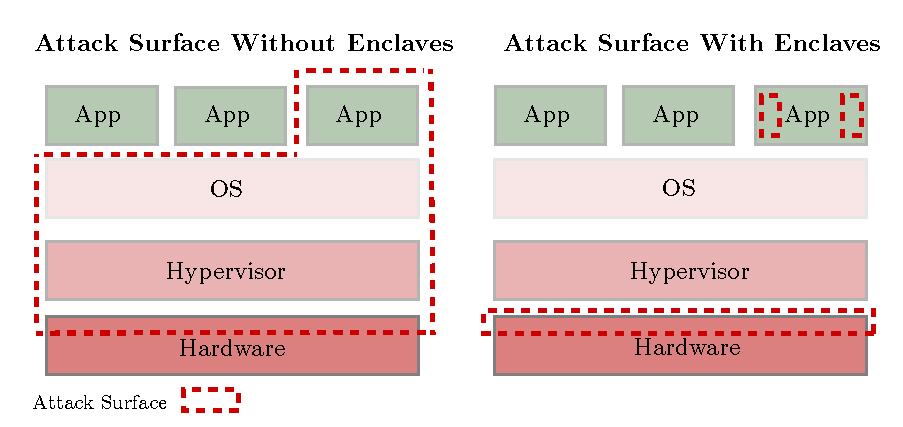
\includegraphics[width=\textwidth]{enclave}
	\caption{
		Attack surface with \acrshort{tee}.
		Adapted from \url{sgx101.gitbook.io}.
	}%
	\label{figure:enclave}
\end{figure}


		While \acrshort{tee} is a concept defining an execution environment, specific solutions include a hardware security module (a plug-in device with a protected memory and a crypto-optimized processing unit), an \acrshort{fpga}, and a set of extensions to an existing processor architecture, such as an \acrshort{sgx} for Intel x86 or Secure Encrypted Virtualization \cite{amd-memory-encryption} for AMD\@.
		Of all these, Intel \acrshort{sgx} is the most widely used technology.

		\subsection{\texorpdfstring{\acrlong{sgx}}{Software Guard Extensions}}

			\acrfull{sgx} is a set of instructions for the Intel x86 architecture that allow a user or an \acrlong{os} to define a region of protected memory, called the \emph{enclave}, and interact with it.
			The enclave can only be accessed using the \acrshort{sgx} instructions (i.e, regular \texttt{mov} instruction would not work), and all pages of the enclave are symmetrically encrypted and physically protected.
			\acrshort{sgx} guarantees the integrity and security of the memory pages within the enclave.
			Although the size of enclave memory is very limited, \acrshort{sgx} can use regular \acrshort{ram} by transparently swapping the pages between the trusted and untrusted memory.
			The pages are then encrypted with integrity protection when placed in the \acrshort{ram} (\emph{sealing} in \acrshort{sgx} terms).

			An \acrshort{sgx}-enabled application declares its trusted and untrusted components upfront.
			Trusted part will live entirely in the enclave, while the untrusted part is a normal process that runs within the \acrshort{os}.
			The application has to be digitally signed for the enclave to accept it, and the enclave itself can authenticate to the user via an \emph{attestation} process.
			Conceptually, the simplest \acrshort{sgx} application in an outsourced database system can be seen as a trusted component that operates over sensitive material (e.g., keys, tokens, plaintext user data), a remote trusted client application that communicates with the enclave, and a layer of code that passes requests through (untrusted part of an \acrshort{sgx} application).
			Cipherbase \cite{cipherbase-daas} and StealthDB \cite{stealth-db} are good examples of such approach.

		\subsection{Issues with \acrshort{sgx}}

			\acrshort{sgx}, as the closest instantiation of \acrshort{tee} available, has been extensively targeted.
			The attacks include Foreshadow \cite{foreshadow}, Prime+Probe cache attack \cite{prime-probe-sgx-attack}, an attack from within the enclave \cite{enclave-sgx-attack}, Spectre line of attacks that can bypass \acrshort{sgx} \cite{spectre-sgx-attack}, replay attack \cite{replay-sgx-attack}, Plundervolt attack \cite{plundervolt-sgx-attack}, Load Value Injection attack \cite{lvi-sgx-attack} and SGAxe attack \cite{sgaxe-sgx-attack}.
			Due to its many security issues, \acrshort{sgx} has been officially discontinued.\footnote{As of $11^\text{th}$ Generation Intel Core processor.}

			Besides the attacks against the \acrshort{sgx}, the design itself has a number of restrictions.
			First of all, the enclave memory is capped at \SI{128}{\mega\byte}, part of which is occupied by the \acrshort{sgx} control structures, leaving the application about \SI{96}{\mega\byte}.
			\acrshort{sgx} allows the use of external memory pages through the sealing mechanism, but it imposes high overhead of re-encryption and crossing the enclave physical boundary.
			Second, the code execution inside the enclave is significantly slower.
			Third, by design, only the untrusted application component can interact with the \acrshort{os}, for example, make network or storage \acrshort{io} requests.
			Finally, from the security standpoint the enclave is vulnerable against the side-channel attacks, most of all, access pattern leakage.
			Such leakage implies that the normal database application cannot be placed directly in the enclave and be deemed secure, because access pattern has been effectively exploited up to a reconstruction attack \cite{generic-attacks-kellaris}.
			One then has to design the application specifically to conceal the access pattern.
			For example, ZeroTrace \cite{zerotrace} is a variant of PathORAM \cite{path-oram} that is internally oblivious and thus can work in \acrshort{sgx}.
			Oblix \cite{oblix} is another example of a structure that is, in \textcite{oblix} own terms, doubly-oblivious --- internally in how manages memory and registers, and externally in how it interacts with a storage.
